% options:
% thesis=B bachelor's thesis
% thesis=M master's thesis
% czech thesis in Czech language
% english thesis in English language
% hidelinks remove colour boxes around hyperlinks

\documentclass[thesis=B,english]{FITthesis}[2012/10/20]

% \usepackage[utf8]{inputenc} % LaTeX source encoded as UTF-8
% \usepackage[latin2]{inputenc} % LaTeX source encoded as ISO-8859-2
% \usepackage[cp1250]{inputenc} % LaTeX source encoded as Windows-1250

\usepackage{graphicx} %graphics files inclusion
% \usepackage{subfig} %subfigures
% \usepackage{amsmath} %advanced maths
% \usepackage{amssymb} %additional math symbols

\usepackage{dirtree} %directory tree visualisation

\usepackage{algpseudocode}
\usepackage{algorithm}
%\usepackage{algpseudocode}
\usepackage{csquotes}
\usepackage{url}
\usepackage[strings]{underscore}

\interfootnotelinepenalty=10000
\widowpenalty10000
\clubpenalty10000

\DeclareTextCommand{\textunderscore}{OT1}{\leavevmode\vbox{\hrule width.5em height.35mm}}

% % list of acronyms
% \usepackage[acronym,nonumberlist,toc,numberedsection=autolabel]{glossaries}
% \iflanguage{czech}{\renewcommand*{\acronymname}{Seznam pou{\v z}it{\' y}ch zkratek}}{}
% \makeglossaries

\department{Department of Computer Systems}
\title{Analysis of the Rescue File of BestCrypt Volume Encryption}
\authorGN{Jan} %author's given name/names
\authorFN{Vojt{\v e}{\v s}ek} %author's surname
\author{Jan Vojt{\v e}{\v s}ek} %author's name without academic degrees
\authorWithDegrees{Jan Vojt{\v e}{\v s}ek} %author's name with academic degrees
\supervisor{Ing. Josef Koke{\v s}}

\acknowledgements{I would like to express my sincere thanks to my supervisor Ing. Josef Koke{\v s} for his valuable insight and reviews. I would also like to thank Jetico Inc. for allowing me to analyze their product and for promptly fixing disclosed bugs and vulnerabilities. Last but not least, I would like to thank my family for their support. }

\abstractEN{This thesis focuses on reverse engineering and security analysis of a disk encryption application called BestCrypt Volume Encryption. It provides a detailed description of a previously undocumented binary file format used for rescue procedures. Several vulnerabilities and bugs were found during the performed security analysis. Each of those vulnerabilities is discussed in detail and an example of how this vulnerability might affect the security of regular users is given. The author also cooperated with the developers of BestCrypt Volume Encryption in order to fix or at least mitigate those vulnerabilities. A tool that makes it possible to mount encrypted volumes on some Unix-like systems is also presented.}


\abstractCS{Tato pr{\' a}ce je zam{\v e}{\v r}ena na reverzn{\' i} in{\v z}en{\' y}rstv{\' i} a bezpe{\v c}nostn{\' i} anal{\' y}zu programu na {\v s}ifrov{\' a}n{\' i} disku BestCrypt Volume Encryption. Obsahuje de\-tail\-n{\' i} popis doposud nedokumentovan{\' e}ho bin{\' a}rn{\' i}ho form{\' a}tu souboru, kter{\' y} se pou{\v z}{\' i}v{\' a} p{\v r}i z{\' a}chrann{\' y}ch operac{\' i}ch. B{\v e}hem bezpe{\v c}nostn{\' i} anal{\' y}zy bylo naleze\-no n{\v e}kolik zranitelnost{\' i} a z{\' a}vad. V{\v s}echny zranitelnosti jsou podrobn{\v e} pops{\' a}ny a je uveden p{\v r}{\' i}klad, jak{\' y}m tato zranitelnost m\accent23u{\v z}e zas{\' a}hnout b{\v e}{\v z}n{\' e}ho u{\v z}ivatele. Autor tak{\' e} spolupracoval s v{\' y}voj{\' a}{\v r}i BestCrypt Volume Encryption ve snaze, aby tyto zranitelnosti byly opraveny nebo aby byl alespo{\v n} zm{\' i}rn{\v e}n jejich dopad. Sou{\v c}{\' a}st{\' i} pr{\' a}ce je i n{\' a}stroj, kter{\' y} umo{\v z}{\v n}uje p{\v r}ipojit za{\v s}ifrovan{\' e} svazky disk{\r u} na n{\v e}kter{\' y}ch opera{\v c}n{\' i}ch syst{\' e}mech zalo{\v z}en{\' y}ch na Unixu.}
\placeForDeclarationOfAuthenticity{Prague}
\keywordsCS{{\v s}ifrov{\' a}n{\' i} disku, reverzn{\' i} in{\v z}en{\' y}rstv{\' i}, BestCrypt Volume Encryption, kryptografie}
\keywordsEN{disk encryption, reverse engineering, BestCrypt Volume Encryption, cryptography}
\declarationOfAuthenticityOption{1} %select as appropriate, according to the desired license (integer 1-6)

\begin{document}
	
	% \newacronym{CVUT}{{\v C}VUT}{{\v C}esk{\' e} vysok{\' e} u{\v c}en{\' i} technick{\' e} v Praze}
	% \newacronym{FIT}{FIT}{Fakulta informa{\v c}n{\' i}ch technologi{\' i}}
	
	\setsecnumdepth{part}
	\chapter{Introduction}
	
	Disk encryption is an integral part of information security. Companies and individuals use it to lower the chances of unauthorized access to their data. Since many people recognize the value of information and the performance impact of encryption seems to be steadily decreasing, disk encryption software is quite prevalent nowadays. On many mobile devices, disk encryption is now even enabled by default. Some newer versions of Windows feature a built-in disk encryption tool called BitLocker. However, many users opt for third-party software, such as BestCrypt Volume Encryption.
	
	If writing secure code is hard, implementing cryptography securely is even more difficult. In order to lower the number of design flaws and implementation vulnerabilities, it is generally recommended to perform a security analysis. That is precisely the goal of my thesis---to independently analyze the security of BestCrypt Volume Encryption. As an independent security researcher, I stand in a unique position. On one hand, I am able to analyze code from a different perspective than the people who wrote it and I am unrestricted by company policies on what I can publish. On the other hand, since I analyze closed source software, I have to use reverse engineering, which makes my efforts significantly more difficult.
	
	There are three main conceptual goals of this thesis. First of all, I am cooperating with the developers of BestCrypt Volume Encryption. If I find any vulnerability or a bug, I will immediately disclose it to them along with a proposed fix or mitigation. In this way, I hope to make this piece of software more secure for all of its users.
	
	This thesis also aims to educate common users of disk encryption software. The problem with security software is the fact that its regular users are usually unable to assess its security by themselves. Readers of this thesis should be able to understand weaknesses both inherent to disk encryption and specific to BestCrypt Volume Encryption.
	
	Last but not least, I also hope that this thesis will help other security researchers analyze 
	BestCrypt Volume Encryption in the future. The documented contents of the rescue file and the developed tools should save them some time and enable them to focus more on other parts of this disk encryption software.
	
	The first two chapters of this thesis are theoretical. \hyperref[ch:first]{The first one} introduces BestCrypt Volume Encryption along with the cryptography it uses. \Cref{ch:second} describes the techniques I used to obtain the results presented in the next chapters. In \cref{ch:third}, the contents of the rescue file are described in detail with an emphasis on security of the rescue file. \Cref{ch:fourth} contains mostly a description of vulnerabilities that were found during security analysis. Finally, an overview of the tools I developed can be found in \cref{ch:fifth}.
	
	\setsecnumdepth{all}
	\chapter{BestCrypt Volume Encryption}
	\label{ch:first}
	
	BestCrypt Volume Encryption (BCVE) is a Windows application designed for transparent encryption of storage volumes. It helps its users keep confidential data on stolen or lost devices encrypted. BCVE was developed by a Finnish company named \textit{Jetico~Inc.~Oy}, who originally started developing encryption products back in 1993. \textit{Jetico} is still active at the time of writing---BCVE continues to receive both new features and security updates. 
	
	This thesis analyzes only BCVE v.3.72.01 and while most of the results are likely going to be applicable to newer and older versions as well, I will describe undocumented internals of BCVE that might be changed at any time. Similarly, some functionality described in this thesis might not be present in older versions of this program. BCVE also comes in two editions: personal and enterprise. It is not a goal of this thesis to analyze the enterprise edition.
	
	\section{Volume encryption}
	As stated earlier, BCVE encrypts whole volumes at once, making it a volume encryption software. This is only one of many possible approaches to encryption of data stored on a hard disk. Some widely used approaches similar to volume encryption will be listed and briefly described in this section. 
	
	\begin{itemize}
		\item \textbf{Full disk encryption}
		
		Full disk encryption software encrypts all sectors on the physical disk, with the possible exception of the boot sector and up to 63 following sectors. Encryption and decryption are transparent, meaning that the data is decrypted on read operations and encrypted on write operations. Transparent software encryption and decryption is usually implemented in a custom driver.
		
		
		Since full disk encryption encrypts physical disks as a whole, it becomes difficult to decrypt parts of the disk without compromising the security of the rest of the disk. If full disk encryption is used on volumes that reside on multiple hard disks, each disk has to be  encrypted separately. On the upside, full disk encryption is suited for hardware implementation. Hardware full disk encryption is completely transparent to software and can achieve better performance than a software implementation.
		
		
		\item \textbf{Filesystem-level encryption}
		
		Encryption can also be implemented at the filesystem level. Implementations may vary, but usually only the content of files is encrypted, while metadata and the structure of the filesystem itself stay unencrypted. This naturally leads to a variety of security and privacy concerns. But in cases where leaving the metadata in plaintext is an option, filesystem-level encryption can be more lightweight because many filesystem operations can be performed without incurring the encryption overhead.
		
		Filesystem-level encryption is most notably implemented inside NTFS as a feature called Encrypting File System.
		
		\item \textbf{Container-based encryption}
		
		Container-based encryption software packs a whole directory structure into a single encrypted file called a container. This container can then be mounted as a volume for transparent read and write access. The advantage of this approach is its adjustable scope of encryption---it only encrypts the files that the user selected without affecting the performance of the rest of the system. Containers are also easily moved from one machine to another. On the other hand, not everything can be encrypted within a container---including but not limited to system files, paging files, and hibernation files.
		
		Container-based encryption was implemented in the discontinued application TrueCrypt. Other implementations include a fork of TrueCrypt, VeraCrypt, or  BestCrypt Container Encryption. 
		
		\item \textbf{Volume encryption}
		
		Volume encryption works similarly to full disk encryption---the biggest difference is that instead of encrypting physical disks, volumes (logical disks) are encrypted. This means that encryption is not limited to simple volumes---for example on Windows systems users can encrypt spanned, striped, mirrored, and RAID-5 volumes across multiple disks too. While this can be done by using full disk encryption as well, volume encryption tends to be more convenient and generally easier to use.
		
		If the encrypted volume contains a boot loader or anything essential for the process of booting up, volume encryption software has to start running even before the boot loader. That usually means replacing the boot sector with its own code, which later passes control back to the original boot loader. This is a complex process and it can cause significant errors when implemented incorrectly. Therefore, there is a need for a robust implementation of rescue procedures for solving potential errors. This is a drawback that volume encryption shares with full disk encryption.
		
		Besides BCVE, volume encryption is also implemented in Windows as a feature called BitLocker.
		
		\item \textbf{Partition encryption}
		
		Partition encryption software encrypts just a single disk partition. This is usually more flexible than full disk encryption, since access can be given to each partition separately. Partition encryption also allows users to shrink a partition before encryption in order to speed up initial encryption. Note that full disk encryption and encryption of a single partition spanning the entire disk do essentially the same thing.
		
		Partition encryption can also be thought of as a subset of volume encryption. Volume encryption software can encrypt volumes consisting of a single partition too.
	\end{itemize}
	
	\section{Overview of BestCrypt Volume Encryption}
	Even though BCVE features a command-line interface, not all its functionality is exposed through it. Therefore, this section will describe BCVE's GUI and walk the reader through some of the use cases relevant to the rest of this thesis. 
	
	After installing and running BCVE, the user is presented a GUI similar to the Microsoft Management Console's snap-in Disk Management (see \-\Cref{fig:bcvemmc}). However, while Disk Management displays information about disks and volumes in general, BCVE's GUI focuses more on items relevant to volume encryption. Some information present in Disk Management is not displayed in BCVE. This includes unallocated space, disks containing no volumes, or CD/DVD discs. 
	
	
	
	\subsection{Encryption and decryption of a volume}
	
	After selecting a volume to encrypt, the user chooses an encryption algorithm. AES, RC6, Serpent, and Twofish are the only choices, with AES being selected by default. All of them use the XTS mode of operation with a 256-bit data encryption key and a 256-bit tweak key. The user also selects whether she wants to format the volume and whether she wants to encrypt all sectors or just perform minimal initial encryption\footnote {Minimal initial encryption is going to be described in \cref{subsec:minimal}.}. If the user wants to format the volume, the format is done after the initial encryption by a standard Windows tool using transparent encryption. The user is also asked to input a new master password. The password must be at least 8 characters in length and must contain only 7-bit ASCII characters.
	
	\begin{figure}
		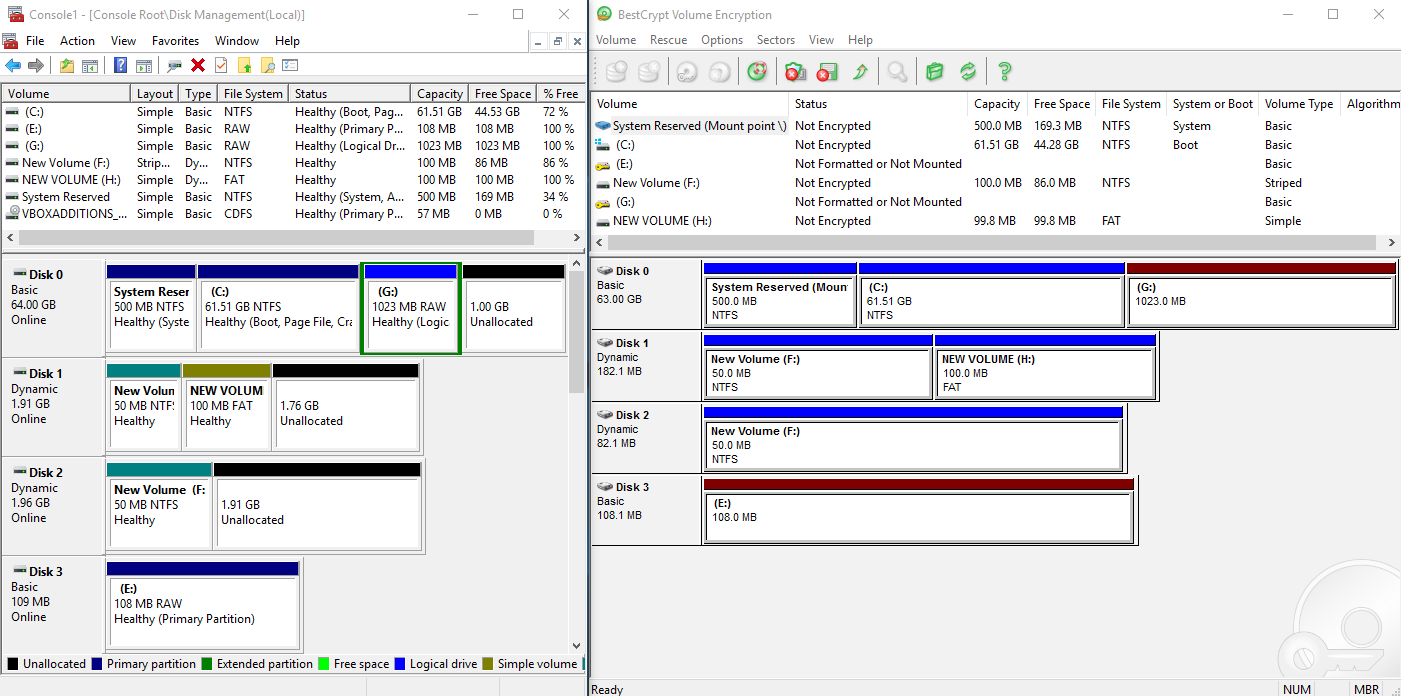
\includegraphics[width=\linewidth]{bcve_mmc_ss.png}
		\caption[Similarity between BCVE's and Disk Management's GUIs]{A screenshot of Microsoft Management Console's snap-in Disk Management (left) and of BestCrypt Volume Encryption (right)}
		\label{fig:bcvemmc}
	\end{figure}
	
	After filling out the password, another dialog is presented to the user, asking her to move her mouse or input random keystrokes in order to collect additional entropy. After some amount of randomness has been collected, BCVE proceeds to actually encrypt the volume. When the encryption is over, the user is informed that the rescue file has been updated and is asked to back it up. 
	
	The process of decryption is simple. The user is asked for the master password and has to confirm that she really wants to decrypt the volume. If all goes well, the volume is decrypted.
	
	\subsection{Mounting and dismounting a volume}
	
	To successfully mount a volume, all the user has to do is input a correct password. This starts the transparent encryption and decryption of all reads and writes to the sectors on the encrypted volume. Once the volume is mounted, the user can work with it just like with any other volume. 
	
	Dismounting doesn't require any password. However, BCVE will not dismount a volume if there are any open handles to a file stored within that volume. Jetico, the developer of BCVE, claims, that after a successful dismount, ``access to plain data from the volume will be impossible'' \cite{bcve_help}.
	
	\subsection{Passwords in BCVE}
	
	A typical BCVE user never sees her encryption key. Unless some additional feature (such as two-factor authentication) is enabled, a password is all the user needs to mount or decrypt a volume. Since passwords might get compromised, BCVE allows to change the master password. To do that, the user has to enter the old master password as well as the new one. The change of the master password is immediately finished. That makes me assume that BCVE does not re-encrypt the volume after a password change. 
	
	In addition to the master password, there are also up to four additional passwords per volume. Anyone with a knowledge of the master password is able to create, modify, and delete them. Additional passwords can be used to mount an encrypted volume. However, BCVE does not allow its users to permanently decrypt a volume using an additional password.
	
	\section{Additional features}
	
	BCVE also offers a fair amount of other features. Some of them are going to be discussed in this section.
	
	\subsection{Pre-boot authentication}
	
	Pre-boot authentication is used only if boot or system volumes are encrypted. Boot volume is the volume where most of the operating system files are stored~\cite{system_boot}, \cite{russinovich}. It typically contains a folder called ``Windows''. System volume is located on an active partition and contains the Boot Manager and Boot Configuration Data. BitLocker might also write to the system volume. 
	
	Both volumes are needed during booting and therefore must be accessible before Windows starts booting. BCVE solves this by overwriting the boot sector with its own code. This way it makes sure that the firmware passes control directly to it \cite{ibm_booting}. BCVE then proceeds to load the rest of its code and prompts the user for a password. After entering a correct password, it starts the transparent encryption and decryption of boot/system volumes and passes control back to the original first stage boot loader. Pre-boot authentication is described in more detail in \cite{hornak}.
	
	\subsection{Minimal initial encryption}
	\label{subsec:minimal}
	
	Minimal initial encryption is a feature designed for speeding up the process of initial encryption. BCVE first ensures that it will transparently encrypt and decrypt all subsequent reads and writes to the volume and asks the user to format it\footnote{BCVE therefore initially only encrypts sector writes done during the format.}. Note that if only a quick format is performed, some sectors on the volume will stay unencrypted. This leads to potential security issues if the volume already contained confidential data. It also lets an adversary guess the amount of used space on the volume \cite{bcve_help} because the yet unencrypted sectors are likely to be distinguishable from random data. BCVE offers the user to overwrite the whole volume with pseudorandom data before the encryption starts to solve those problems\footnote{This is done at the expense of initial encryption speed.}.
	
	\subsection{Two factor authentication}
	
	In addition to passwords (something users know), the encrypted volumes can be protected with a second authentication factor: \textit{SafeNet eToken Pro}\footnote{https://safenet.gemalto.com/multi-factor-authentication/authenticators/pki-usb-authentication/etoken-5110-usb-token/} (something users have). If two-factor authentication is enabled, users have to both connect this hardware security token to a USB port and type a correct password to get access to the volume. Both are then used to derive encryption keys. The token is only used for key derivation and so it is not needed anymore after the volume has been mounted. In version 3 of BCVE, two-factor authentication is available with any conventional removable disks too.
	
	\subsection{AES instruction set}
	
	Given the widespread use of AES, Intel added six new instructions offering hardware support for AES to the x86 instruction set \cite{aesni}. BCVE makes use of those instructions if they are available to the processor it is running on. This results in about 30\% increase in the overall throughput of disk operations~\cite{bcve_help}. The use of the AES instruction set can be turned off in order to fall back to a pure software implementation of AES. 
	
	\section{Cryptographic primitives used}
	
	Given the fact that BCVE is an encryption application, one might expect it to use a large amount of cryptographic primitives. Indeed, BCVE makes use of both symmetric and asymmetric encryption, hash functions, and cryptographically secure PRNGs. While asymmetric encryption is used in the enterprise edition of BCVE for secure communication with the Jetico Central Manager, symmetric encryption is vital to both editions of BCVE---it is used to actually encrypt the volume. 
	
	BCVE offers its user a choice of four symmetric block ciphers: AES, RC6, Serpent, and Twofish. 
	All of them were finalists in the AES process\footnote{The AES process was organized by NIST and its goal was to set a new standard block cipher and to call this cipher AES. There was a total of 15 ciphers submitted, with five of them making it to the second round (I refer to those as AES finalists). Eventually, a cipher called Rijndael was chosen to become AES. All ciphers submitted had to operate on blocks of 128 bits and support key sizes of 128, 192, and 256 bits.} and are implemented in BCVE with the largest possible key size of 256 bits. During reverse engineering, I have found  that three more symmetric block ciphers are supported for already encrypted volumes: CAST-128, GOST, and Blowfish. This section is meant to provide a quick introduction to the individual cryptographic primitives used as well as the XTS mode of operation.
	
	\subsection{AES}
	
	The Advanced Encryption Standard \cite{rijndael} is a block cipher published by Vincent Rijmen and Joan Daemen in 1998. Originally named Rijndael, it won its name after a rigorous assessment in the Advanced Encryption Standard process \cite{aes}. Unlike many previous block ciphers, AES does not use a Feistel network \cite{feistel}. Instead, it consists of several rounds of substitution and permutation and it was designed for efficient implementation in both hardware and software. 
	
	\subsection{RC6}
	
	Rivest cipher 6 \cite{rc6} is a block cipher based on its extremely simple predecessor named RC5. It is fully parameterized, meaning the size of the key and the number of rounds can be adjusted. But since certain versions of RC6 were submitted to the AES process, the parameters in those versions are the ones most widely used in practice. RC6 is a proprietary algorithm and it was patented by \textit{RSA Data Security,~Inc.}
	
	\subsection{Serpent}
	
	Serpent \cite{serpent} is another AES finalist block cipher. Since parts of its design were similar to DES, the extensive research of DES was partially applicable to Serpent. Serpent was designed for maximum security. While the authors considered 16-round Serpent to be sufficiently secure \cite{serpent}, the published version of Serpent used 32 rounds. This way, Serpent was expected to withstand decades of cryptanalysis. 
	
	Serpent ended up second in the AES process. The most significant drawback of Serpent was its performance. It was slow compared to the other AES finalists~\cite{aes_perf}.
	
	\subsection{Twofish}
	
	Twofish \cite{twofish} is a block cipher published by Bruce Schneier et al. The design of Twofish is similar to its predecessor called Blowfish. It uses a Feistel network and its S-boxes are key-dependent. Like RC6, the size of the key can be variable, but it is most commonly implemented with key sizes of either 128, 192, or 256 bits. Twofish was designed to be efficient on most computer architectures and in hardware. It also allows several performance trade-offs between encryption speed and key schedule speed as well as between encryption speed and the amount of memory used.
	
	\subsection{64-bit block ciphers}
	
	While all the block ciphers described above were AES finalists and therefore had a 128-bit block size\footnote{This was one of the requirements in the AES process.}, the following three block ciphers encrypt blocks of 64 bits. The problem with 64-bit block ciphers is that they are in some cases vulnerable to collision attacks \cite{sweet32}. This might also be the case with BCVE, since the same encryption key is used to encrypt a whole volume\footnote{Due to the birthday paradox, the probability of a collision is non-negligible for larger volumes.} and an adversary can potentially make the user store their own chosen plaintext blocks on the volume\footnote{The adversary can also try to guess the contents of some sectors.}. In practice, those attacks are prevented by using the XTS or LRW mode of operation, so they might only be applicable to older volumes using CBC mode. However, it is still generally recommended to steer away from using 64-bit block ciphers. This is exactly what BCVE is doing, since it does not allow the user to choose those ciphers for newly encrypted volumes.
	
	\subsection{Blowfish}
	
	Blowfish \cite{blowfish} is a 64-bit block cipher designed by Bruce Schneier. It is structured as a Feistel network and uses key-dependent S-boxes. Its key schedule algorithm is relatively slow and it needs more than four kilobytes of memory for encryption. While those properties might make Blowfish impractical in some cases, they are also useful for the construction of password hashing functions such as bcrypt. 
	
	\subsection{CAST-128}
	
	CAST-128 \cite{cast128} is 16-round Feistel cipher notably used in GPG and PGP. A related cipher, CAST-256, was submitted to the AES process, but did not make it among the AES finalists. CAST-128 encrypts 64-bit blocks and does not support keys larger than 128 bits.
	
	\subsection{GOST 28147-89}
	
	GOST \cite{gost} is a Feistel cipher developed by the KGB in the 1970s. It was declassified after the dissolution of the Soviet Union. An interesting feature of GOST is that no S-boxes were originally published. Users of GOST had to generate their own. However, in order to avoid weak S-boxes, a standard one was specified in 2015. 
	
	\subsection{SHA-2}
	
	SHA-2 \cite{sha2} is a family of cryptographic hash functions designed by the NSA. It is a successor of SHA-1---a hash function whose collision was published in 2017~\cite{shattered}. SHA-2 is also a predecessor of a differently designed hash function SHA-3 (Keccak). There are six SHA-2 functions in total, mostly differing in the size of their digests. SHA-2 is widely used in cryptographic protocols such as TLS, SSH, IPSec and in many others. Because of its prevalence and its low memory usage, many dedicated ASICs have been built for SHA-2 hash functions \cite{sha_asic}. They usually outperform software implementations by a significant margin.
	
	\subsection{XTS mode of operation}
	
	A block cipher defines just a transformation of a fixed size block to another fixed size block. To encrypt and decrypt data of arbitrary length, a mode of operation is used on top of a block cipher. Modes of operation are independent of block ciphers and therefore any combination of a block cipher and a mode of operation can be used. There are many modes of operation, but for the purpose of disk encryption, XTS is recommended in an IEEE standard \cite{ieee_xts}.
	
	XTS is a tweakable \cite{tweak} mode of operation. It is based on the XEX mode and it provides special handling for encrypting data whose size is not a multiple of the cipher block size. In the context of BCVE, the disk sector size is always a multiple of the cipher block size, so XEX and XTS are very similar in function. Basically, the only difference is that XEX uses the same encryption key to generate a tweak and to encrypt plaintext blocks.
	
	XTS uses two different keys for encryption. The first key (I am going to refer to this key as the tweak key from now on) is used together with a position of the block to derive the tweak. During encryption, a plaintext block is first XORed to the tweak, then encrypted with a block cipher using the second key (this is going to be called the data key from now on) and finally XORed again with the tweak to obtain the final ciphertext.
	
	\begin{algorithm}
		\caption{XTS encryption
			\label{alg:xtse}}
		\begin{algorithmic}[1]
			\State $T\gets E_{k_1}(i) \bigotimes \alpha ^ j $
			\State $C\gets E_{k_2}(P \oplus T) \oplus T $
		\end{algorithmic}
	\end{algorithm}
	
	In the XTS algorithms, $k_1$ denotes the tweak key, $k_2$ is the data key, $i$ is the sector number, $j$ is the position of the block within a sector, $P$ is the plaintext block, $C$ is the ciphertext block, $\alpha$ is 2. $E$ is block cipher encryption, $D$ is block cipher decryption, $\oplus$ is the bitwise XOR operator, and $\bigotimes$ is multiplication in $GF(2 ^{block\_size})$.
	
	Decryption is straightforward---a ciphertext block is first XORed to the tweak, then decrypted with a block cipher using the data key and finally XORed again with the tweak. Note that the value of the tweak is different for each block position on the disk. 
	
	\begin{algorithm}
		\caption{XTS decryption
			\label{alg:xtsd}}
		\begin{algorithmic}[1]
			\State $T\gets E_{k_1}(i) \bigotimes \alpha ^ j $
			\State $P\gets D_{k_2}(C \oplus T) \oplus T $
		\end{algorithmic}
	\end{algorithm}
	
	Please note that using XTS does not prevent an adversary with recurring access to the encrypted volume from observing if a block has changed its content or not. An adversary can also revert a block to a previously observed content or completely randomize a plaintext block by flipping a bit in the corresponding ciphertext block. Since XTS does not use any integrity mechanisms, any change to an encrypted volume is undetectable by the encryption application.
	
	\section{Rescue procedures}
	
	An inherent risk in disk encryption is a possibility of data loss. Passwords might get forgotten, hard drives might get corrupted, modified boot loaders might crash, critical data might get accidentally overwritten, etc. BCVE offers its users a number of rescue procedures to minimize this risk. However, in order to be able to use those rescue procedures, the user has to first save and back up the rescue file. Rescue procedures then try to use data stored in the rescue file to recover from a wide variety of possible errors.
	
	\subsection{Rescue file}
	BCVE asks the user to save the rescue file after any major change is performed to a volume. Those changes include encryption/decryption of a volume, change of the master password, or setting up two-factor authentication. In fact, the rescue file is stored in the installation directory of BCVE\footnote{It is possible to reconfigure BCVE to save the rescue file automatically elsewhere.} and it is updated automatically. If the user wishes to back up the rescue file, it is simply copied to a user-chosen location. 
	
	\label{subsec:accessible}
	
	The point of the rescue file is that it is accessible in case of failure. Therefore, it is generally not a good idea to store the rescue file on an encrypted volume. Consequently, the rescue file is usually more accessible to potential adversaries. It is essential, that access to the rescue file does not make it easier for an adversary to decrypt a volume. Jetico, the developer of BCVE, claims that ``information inside Rescue File is encrypted exactly in the same way as on volumes, so there is no risk that someone	not knowing proper passwords can use the file'' \cite{bcve_help}. One of the main goals of my thesis is to verify this statement.
	
	The rescue file stores 0xCF4 bytes of data per encrypted volume. Since it does not appear to contain any meaningful ASCII readable strings, the format of the rescue file is most likely binary. About half of the file is filled with zero bytes. This suggests that some parts of the rescue file are filled conditionally or that they are reserved for future use. After a successful decryption of a volume, rescue data for that volume is still left in the rescue file. It is overwritten when the decrypted volume is encrypted again.
	
	To back up the rescue file, a user can either select \textbf{Rescue-\textgreater{}Save Rescue Data} in the menu bar or back it up manually by copying the file. Recovery decryption is run by selecting \textbf{Rescue-\textgreater{}Decrypt with Rescue File}.
	
	\subsection{Rescue bootable medium}
	
	If a system/boot volume is encrypted, BCVE no longer asks the user to save the rescue file. Instead, it suggests creating a bootable recovery medium. This medium can be a CD/DVD, a USB, or a floppy disk. The bootable medium is needed because Windows won't boot without a mounted system/boot volume and therefore any errors have to be resolved before passing control to the Windows boot loader.
	
	Note that the bootable medium contains the rescue file \cite{bcve_help}, so any analysis performed on the rescue file applies to any rescue bootable medium too. Another thing worth pointing out is that even when BCVE does not allow the user to back up the rescue file using the GUI, its contents are still being updated in the background.
	
	
	\chapter{Reverse engineering}
	\label{ch:second}	
	
	Reverse engineering is the process of analyzing anything man-made in order to learn details of its design and implementation. It can be applied to both hardware and software. While hardware reverse engineers actually study tangible pieces of hardware, software reverse engineers usually deal with executable code. This can be machine code to be executed directly by a CPU, bytecode to be processed, or source code of a script to be interpreted. The findings described in this thesis are going to be mostly obtained by performing software reverse engineering of machine code compiled for the x86 instruction set architecture.
	
	\section{Applications of software reverse engineering}
	
	Reverse engineering used to be closely associated with military or commercial espionage \cite{reveng_origin}. However, there are many more reasons for performing reverse engineering nowadays. Note that since reverse engineering is just a tool, it can be used by both people with good and malicious intents.
	
	\begin{itemize}
		\item \textbf{Malware analysis}
		
		Reverse engineering is useful for finding out whether a piece of software is malicious or not. If it is, malware analysts can also gather more information to detect similar pieces of malware in the future. In some cases, analysts can find an exploited zero-day vulnerability or take advantage of flaws found in malware (e.g., to write ransomware decryptors). This type of reverse engineering is often made harder by the use of obfuscation and anti-debugging tricks.
		
		\item \textbf{Achieving interoperability}
		
		Reverse engineering can be used for system integration or replacement of legacy systems if there isn't sufficient documentation available. It is needed if the original developers of the system to be integrated can't be reached or do not wish to cooperate. Reverse engineering is also a way of documenting unknown file formats or network protocols \cite{reveng}. Examples of the use of reverse engineering for achieving interoperability include ReactOS\footnote{https://www.reactos.org/}, Samba\footnote{https://www.samba.org/}, and Wine\footnote{https://www.winehq.org/}.
		
		\item \textbf{Security analysis}
		
		Software vulnerabilities can be found by means of reverse engineering. Based on the intentions of the reverse engineer, found vulnerabilities are usually either reported\footnote{The most recommended way to do this is ``responsible disclosure''. It means giving developers a certain amount of time to patch the vulnerability before publishing it.} and fixed or attempted to be exploited. Security analysts might also look for backdoors or try to assess software quality.
		
		\item \textbf{Reverse engineering of competitors' products}
		
		There are several reasons why companies might be interested in analyzing their competitors' products. They might want to confirm suspicions that it uses their software without an appropriate license or infringes on one of their patents. Examining the product can also provide them with valuable information that they might use to improve their own product. Note that this is often done illegally.
		
		\item \textbf{Removal of copy protection}
		
		Copy protection mechanisms are built to prevent the unauthorized reproduction of copyrighted work. Software pirates try to understand and locate those mechanisms by means of reverse engineering in order to remove them. It is considered almost impossible to completely prevent a determined and skilled attacker who is given enough time from defeating a copy protection mechanism \cite{copy_protection}, \cite{copy_protection2}.
		
	\end{itemize}
	
	\section{Reverse engineering of binary file formats}
	
	The main benefits of binary file formats are efficient parsing and space saving. On the other hand, their human-readability is much lower than that of text file formats. Any sequence of bytes can be interpreted in multiple ways, so completely reverse engineering a binary file format is often impossible without having access to an application that uses the examined file format. Reverse engineering can be made even more difficult by compression, encryption, or obfuscation. However, it is sometimes possible to infer some information about a binary file format just by observing examples, since they might contain some identifiable elements. Those elements include strings of text, pieces of code, offsets within the file, magic numbers, sizes of data blocks, checksums,~etc. Moreover, those elements often form arrays or any other data structures. Many encoding schemes are also easy to identify and a high Shannon entropy~\cite{shannon} of data blocks might suggest that they are compressed or encrypted.
	
	The ability to reverse engineer applications that use the file format helps a lot. It is possible to locate procedures that read or write to the file by observing either system calls or library functions. Once those procedures are located, they are a good starting point for reverse engineering. The procedures reading the file usually perform some kind of parsing and the procedures writing to the file should only write data adhering to the file format. More reverse engineering can then be performed to figure out where does the data written to the file come from and what is the data read from the file used for. 
	
	An application handling the analyzed files can also be used without actually reverse engineering its code. One can perform small edits in the application and observe corresponding changes in the analyzed file. Likewise, one can edit the analyzed file and see if it changed the behavior of the application. Letting the application generate a file that is as simple as possible can also be helpful for analysis.
	
	An important thing to keep in mind is that completely reverse engineering a binary file format is a difficult task. Its contents might differ based on the version and edition of the application using it and some parts of it might be obscure and only used rarely. Reverse engineering complex proprietary file formats, such as Microsoft's DOC, therefore requires a lot of work.
	
	\section{Legality of reverse engineering}
	
	Performing reverse engineering is under many circumstances barely legal or outright illegal. Specific cases naturally depend on the jurisdiction used. I will discuss reverse engineering under EU law in this section. 
	
	Software reverse engineering is covered in \textit{Directive 2009/24/EC of the European Parliament and of the Council of 23 April, 2009 on the legal protection of computer programs} \cite{law}. It contains the following paragraph: 
	
	\begin{displayquote}
		The unauthorised reproduction, translation, adaptation or transformation of the form of the code in which a copy of a computer program has been made available constitutes an infringement of the exclusive rights of the author. Nevertheless, circumstances may exist when such a reproduction of the code and translation of its form are indispensable to obtain the necessary information to achieve the interoperability of an independently created program with other programs. It has therefore to be considered that, in these limited circumstances only, performance of the acts of reproduction and translation by or on behalf of a person having a right to use a copy of the program is legitimate and compatible with fair practice and must therefore be deemed not to require the authorisation of the rightholder. An objective of this exception is to make it possible to connect all components of a computer system, including those of different manufacturers, so that they can work together. Such an exception to the author's exclusive rights may not be used in a way which prejudices the legitimate interests of the rightholder or which conflicts with a normal exploitation of the program.
	\end{displayquote}
	
	Please note that the term \textit{interoperability} is defined very broadly in \cite{law}. How to determine whether a specific application of reverse engineering is legal or not is therefore sometimes unclear and relies on an interpretation of this term.
	
	
	Reverse engineering of software is also often explicitly prohibited in an end-user license agreement. This is also the case with BCVE. Please note that Jetico, the developer of BCVE, granted me permission to perform reverse engineering of BCVE and to publish results of my security evaluation. Such an explicit permission overrides the standard end-user license agreement.
	
	\section{Tools used}
	
	Reverse engineers typically use tools such as disassemblers, debuggers, or decompilers. A brief description of tools used for my thesis is presented in this section.
	
	\subsection{IDA}
	
	The Interactive Disassembler (IDA) is a multi-platform proprietary disassembler with support for many instruction sets and executable file formats. It provides a debugger for both local and remote debugging of various types of executables. IDA is scriptable with either Python or its own custom scripting language called IDC. The developer of IDA, Hex-Rays, also offers a decompiler that is integrated into IDA.
	
	Increasing productivity is one of design goals of IDA. It attempts to present a graph-based view of disassembled instructions. This allows reverse engineers to examine the analyzed function's structure and to quickly identify loops and error handling. IDA is also able to recognize and name many standard library functions generated by well-known compilers. All variables and parameters can be given custom names and comments can be entered. IDA saves all information about the analyzed executable in its own database format, which can then be shared with other reverse engineers. IDA is also designed to be extensible and allows its users to create custom plugins for additional functionality. Hex-Rays organizes an annual plugin contest and rewards the most innovative ones.
	
	\subsection{VirtualBox}
	
	VirtualBox is an open-source virtualization product for x86 computers originally developed by Innotek. It runs on most modern desktop operating systems and allows the creation of guest virtual machines that can run a wide range of operating systems too. If the host processor supports hardware-assisted virtualization, VirtualBox can take full advantage of it. VirtualBox also offers a lot of features, such as shared folders, shared clipboard, snapshots, multiscreen support, or virtual USB controllers. Virtualization is especially useful in software development as it allows developers to share the same environment by cloning and taking snapshots.
	
	For the purposes of reverse engineering, virtualization is convenient for kernel debugging. One does not have to worry about breaking their system and can in case of failure just revert the virtual machine to the last snapshot. Kernel debugging of virtual machines is also harder to detect from within the guest, since the debugger is running on the host system. The ability to easily create virtual disk images comes in handy for analyzing volume encryption software.
	
	\subsection{Hiew}
	
	Hiew is a Windows hex editor specialized in editing executable files, such as PE or ELF files. It parses and shows their headers and displays not only offsets within the file but also expected virtual addresses after process loading. Hiew can edit files in text, hex, or disassembly mode. It supports search functions as well as advanced editing, such as assembling instructions, copying data blocks, or XORing data blocks.
	
	\subsection{Active@ Disk Editor}
	
	Active@ Disk Editor is a tool for displaying and editing raw disk sectors. Contents of physical disks, partitions, or volumes can be viewed. It allows searching for an occurrence of a sequence of bytes and decodes contents of key sectors, such as MBR or NTFS boot sector.
	
	\chapter{Rescue file contents}
	\label{ch:third}
	
	This chapter contains a detailed description of the rescue file format. While the primary goal is to analyze the security implications of the rescue file format, this chapter might also be prove to be useful for ordinary users of BCVE. They can now examine the contents of their own rescue files before they back them up for recovery purposes. Note that some users might choose to store their rescue files on an unencrypted disk, in the cloud, or even share their rescue files with other people. In such cases, they are now able to assess the potential security risk for themselves.
	
	Special attention is going to be paid to answering the following questions in particular:
	
	\begin{itemize}
		\item \textbf{Does the rescue file leak any sensitive information?}
		
		As discussed in \cref{subsec:accessible}, the rescue file is usually more accessible to a potential adversary than the encrypted volume itself.  Consequently, just reading the rescue file should not give an adversary any information that might significantly compromise security of corresponding BCVE users.
		
		\item \textbf{Are encryption keys stored securely?}
		
		Since the user authenticates with a password, BCVE has to be able to derive encryption keys just from the password and the rescue file. An adversary should not be able to obtain the encryption keys unless he correctly guesses a password. Usually, individual data items can be stored in plaintext (accessible to anyone), encrypted (accessible to anyone knowing a secret key), or hashed with a one-way hash function (accessible to anyone able to guess the plaintext content). Each data item in the rescue file should be stored in an appropriate way.
		
		\item \textbf{Is there anything missing from the rescue file?}\nopagebreak{}
	
		
		The rescue file is supposed to store all the information needed to perform rescue decryption of a volume. If any important data item was missing, rescue decryption could potentially fail and the user would consequently lose access to her data.
		
		\item \textbf{Does BCVE handle the rescue file safely?}
		
		I decided to analyze not only the rescue file contents but also the way BCVE uses the rescue file. It is in my opinion equally important, since an adversary is in some cases able to tamper with the rescue file and trick a user into using this tampered rescue file for rescue procedures. A vulnerability in the code responsible for reading the rescue file could potentially be exploited with a specially crafted rescue file.
		
	\end{itemize}
	
	The rescue file contains an array of structures 0xCF4 bytes long. Each of those structures (I will be referring to them as \verb|RECOVERY_STRUCTs| from now on) contains rescue information relevant to a single encrypted volume. 
	
	\newcommand{\TextUnderscore}{\rule{.5em}{0.5pt}}
	\section{RECOVERY\textunderscore{}STRUCT contents}
	
	Most of the rescue file contents described in this chapter were identified by reverse engineering BCVE. My efforts were significantly simplified by information found in Hor{\v n}{\' a}k's thesis that studied BCVE's boot loader \cite{hornak}. The contents of the \verb|KEY_AND_HASH| structure are described there along with the secondary key derivation algorithm. Parts of the \verb|KEY_STRUCT| structure are also described there.
	
	After I finished reverse engineering the rescue file format, BCVE's support team shared with me a header file containing \verb|RECOVERY_STRUCT's| definition. I used it to verify the correctness of my previous findings and also started using identifiers found in there. The header file definition also listed items related to EFI and items specific to the enterprise edition of BCVE that I did not reverse engineer beforehand. 
	
	Each of the following subsections is meant to describe a single data item found in the \verb|RECOVERY_STRUCT| (\Cref{tab:recstruct}).
	
	\begin{table}
		\centering
		\begin{tabular}{| l | l | c | l |} 
			\hline
			Offset & Size & Description & Encrypted \\
			\hline \hline
			0x0  & 0x10  & Rescue file signature & No	\\
			\hline
			0x10 & 0x200 & Array of up to eight \verb|KEY_STRUCTs| & No\\ 
			\hline
			0x210 & 0x200 &  \verb|KEY_AND_HASH_PUBKEY_MASTER| & Yes\\ 
			\hline
			0x410 & 0x4 &  Number of disk extents & No\\ 
			\hline
			0x414 & 0x4 &  Decrypted volume flag & No\\ 
			\hline
			0x418 & 0x8 &  Starting offset of the first disk extent & No\\ 
			\hline
			0x420 & 0x8 &  Size of the first disk extent & No\\ 
			\hline
			0x428 & 0x10 & Disk signature of the first disk extent & No\\ 
			\hline
			0x438 & 0x40 & MBR Signature on an EFI disk & No \\ 
			\hline
			0x478 & 0xC & Location of UEFI dummy files  & No\\ 
			\hline
			0x484 & 0x198 & Reserved  & No\\ 
			\hline
			0x61C & 0x8 & Timestamp  & No\\ 
			\hline
			0x624 & 0x4 & Flags  & No\\ 
			\hline
			0x628 & 0x200 & Encrypted first sector & Yes \\ 
			\hline
			0x828 & 0x60 & Master password \verb|KEY_AND_HASH| & Yes \\ 
			\hline
			0x888 & 0x60 & Administrator password \verb|KEY_AND_HASH| & Yes  \\ 
			\hline
			0x8E8 & 0x1 & Mode of operation & No \\ 
			\hline
			0x8E9 & 0x1 & Block cipher identifier & No \\ 
			\hline
			0x8EA & 0x1 & IsSystemVolume flag & No  \\ 
			\hline
			0x8EB & 0x1 & IsBootVolume flag & No   \\ 
			\hline
			0x8EC & 0x8 & Salt & No   \\ 
			\hline
			0x8F4 & 0x200 & Original boot sector & No   \\ 
			\hline
			0xAF4 & 0x1B0 & \verb|ADDITIONAL_PASSWORDS|  & Partially  \\ 
			\hline
			0xCA4 & 0x50 & Reserved & No \\ 
			\hline
			
		\end{tabular}
		\caption{RECOVERY\TextUnderscore{}STRUCT contents}
		\label{tab:recstruct}
	\end{table}
	
	\subsection{Rescue file signature}
	
	File signatures are present in many binary file formats---they are included in a file to indicate its file format. They can then be used as a simple sanity check to avoid processing files that are evidently not in the required file format. A file signature can also be used to determine the type of an unknown file.  
	
	BCVE's rescue file signature is a 16-byte magic number that is being checked any time BCVE accesses the rescue file. This magic number also happens to be a part of the fourth S-box in Blowfish. Since the S-boxes in Blowfish are actually hexadecimal digits of \textit{pi} \cite{blowfish} and the magic number is sixteen bytes long, this is definitely not a coincidence. 
	
	\subsection{KEY\textunderscore{}STRUCT}
	
	Volumes that BCVE encrypts might not be accessible during recovery. That is why BCVE stores information about the structure of the encrypted volume in the rescue file, so that it is able to reconstruct the volume from the disk extents\footnote{Disk extent is a contiguous block on a single disk.} the volume consists of. Definition of the individual disk extents (along with the RAID level the extent is a part of) is stored in a structure called \verb|KEY_STRUCT| (\Cref{tab:keystruct}). There is enough space for eight \verb|KEY_STRUCTs|---if an encrypted volume consists of more than eight disk extents, only information about the first eight disk extents is saved in the rescue file.
	
	\begin{table}
		\centering
		\begin{tabular}{|l | l | c |} 
			\hline
			Offset & Size & Description \\
			\hline \hline
			0x0  & 0x10  & \verb|KEY_STRUCT| signature	\\
			\hline
			0x10 & 0x6 & LBA of the first sector \\ 
			\hline
			0x16 & 0x6 & LBA of the last sector \\ 
			\hline
			0x1C & 0x6 & Total number of encrypted sectors \\ 
			\hline
			0x22 & 0x10 & Disk identifier \\ 
			\hline
			0x32 & 0x1 & Windows disk number \\ 
			\hline
			0x33 & 0x1 & Extent number \\ 
			\hline
			0x34 & 0x1 & Volume type \\ 
			\hline
			0x35 & 0x1 & BIOS disk number \\ 
			\hline
			0x36 & 0x2 & Reserved \\ 
			\hline
			0x38 & 0x6 & LBA of the replaced sector \\ 
			\hline
			0x3E & 0x2 & Reserved \\ 
			\hline
		\end{tabular}
		\caption{KEY\TextUnderscore{}STRUCT contents}
		\label{tab:keystruct}
	\end{table}
	
	\subsubsection{KEY\textunderscore{}STRUCT signature}
	
	It might seem that the presence of the \verb|KEY_STRUCT| signature is unnecessary in
	the \verb|KEY_STRUCT|. But the reason for its existence is that some \verb|KEY_STRUCTs| are also stored directly on disk \cite{hornak}. The presence of this signature is certainly justified when storing critical data structures on raw disks.
	
	\subsubsection{Disk extent position and size}
	
	Disk extent is a contiguous subset of a whole disk. It can be therefore uniquely identified by specifying its start and end offset within a disk. In the \verb|KEY_STRUCT|, both start and end of a disk extent are defined by their sector LBAs\footnote{LBA is a linear addressing scheme often used for identifying disk sectors.}. It might seem redundant to also store the total number of sectors in the disk extent (since it can be computed from the start and end LBAs), but according to BCVE developers the \textit{Total number of encrypted sectors} can be lower than the entire span of the disk extent if the initial encryption was terminated prematurely. 
	
	\subsubsection{Disk identifier}
	
	A disk identifier is used to specify the disk an extent is situated on. If the disk uses the GPT partition style, the identifier is the 16-byte disk GUID. If it uses MBR partitioning, the first four bytes are the MBR signature and the remaining 12 bytes are filled with zero bytes.
	
	\subsubsection{Windows and BIOS disk numbers}
	
	In addition to the disk signature, BCVE also stores two other disk identifiers. The first one is the number Windows assigns to the disk. Windows then makes the raw disk accessible as \textit{\textbackslash\textbackslash.\textbackslash{}PhysicalDriveX}, where \textit{X} is the Windows disk number. 
	
	The second identifier is the number used with BIOS \textit{INT 13h}---a real mode interrupt call used for low-level disk services \cite{int13}. To specify which disk should the interrupt handler operate on, the x86 register DL is set to the 8-bit BIOS disk number value. Note that BIOS disk numbers with the most significant bit cleared are reserved for floppy disks, so hard disk numbering starts from the hexadecimal value of 0x80.
	
	\subsubsection{Extent number}
	
	This byte contains the ordinal number of the disk extent within the volume in the order as it was returned by the \verb|IOCTL_VOLUME_GET_VOLUME_DISK_EXTENTS| control code. With the exception of simple and mirrored volumes (where the order does not matter), the disk extent ordinal number is needed to correctly reconstruct the volume.
	
	The \verb|KEY_STRUCTs| are stored in the rescue file in an ascending order of this extent number so the presence of this field in the rescue file feels a bit redundant. However, as discussed before, the \verb|KEY_STRUCT| is stored in other places as well, where all the \verb|KEY_STRUCTs| might not be stored in the same order.
	
	\subsubsection{Volume type}
	
	Windows allows its users to create dynamic volumes for better performance and/or reliability. This subsection contains the enumeration of all volume types supported by BCVE along with their respective values that are stored in the rescue file.
	
	\begin{itemize}
		\item \textbf{0x01 --- Simple volumes}
		\nopagebreak
		
		Simple volumes contain just a single disk extent. Please note that volumes that consist of multiple disk extents on the same disk are considered to be \textit{spanned volumes} by BCVE even though Windows regards them as \textit{simple volumes}.
		
		\item \textbf{0x02 --- Spanned volumes} 
		\nopagebreak
		
		Spanned volumes link multiple disk extents together. They are useful for enlarging the volume size.
		
		\item \textbf{0x03 --- Striped volumes} 
		\nopagebreak
		
		While spanned volumes concatenate disk extents, striped volumes interleave them in order to increase throughput. Striped volumes can only be created from equally sized disk extents.
		
		\item \textbf{0x04 --- Mirrored volumes} 
		\nopagebreak
		
		Mirrored volumes duplicate data on multiple disk extents in order to achieve fault-tolerance.
		
		\item \textbf{0x05 --- RAID-5 Volumes} 
		\nopagebreak
		
		RAID-5 volumes use three or more disk extents to gain both better reliability and read throughput. Data is stored similarly to striped volumes and parity is computed and split across all disk extents.
		
	\end{itemize}
	
	\subsubsection{LBA of the replaced sector}
	
	The very first sector of an encrypted volume is replaced with BCVE specific data. Its original contents are stored in an encrypted form in the rescue file. If the replaced sector resides on this disk extent, its LBA is stored here. Otherwise, this field is filled with 0xFF bytes.
	
	\subsection{KEY\textunderscore{}AND\textunderscore{}HASH\textunderscore{}PUBKEY\textunderscore{}MASTER}
	
	This data item stores an encryption key used for communication with \textit{Jetico Central Manager}. As it is used only in the enterprise edition of BCVE, I did not analyze its contents.
	
	\subsection{Number of disk extents}
	
	The total number of disk extents that form the encrypted volume is stored here. This is usually equal to the number of \verb|KEY_STRUCTs| present in this \verb|RECOVERY_STRUCT|. But \verb|RECOVERY_STRUCTs| of volumes that consist of more than eight disk extents contain just eight \verb|KEY_STRUCTs|, while this number is set to the actual amount of disk extents.
	
	\subsection{Decrypted volume flag}
	
	After a volume has been permanently decrypted, the \verb|RECOVERY_STRUCT| corresponding to it is not removed from the rescue file. In fact, the only modification done to the rescue file is that the \textit{Decrypted volume flag} is set in order to mark the \verb|RECOVERY_STRUCT| as inactive. This is perhaps done to avoid having to shift the entire contents of the rescue file located after the inactive \verb|RECOVERY_STRUCT|. When a new \verb|RECOVERY_STRUCT| is to be written to the rescue file, BCVE first checks for any inactive \verb|RECOVERY_STRUCTs|. If there is one, BCVE replaces it with the new one. Otherwise, the new \verb|RECOVERY_STRUCT| is appended to the rescue file.
	
	I would consider it more prudent to remove the inactive \verb|RECOVERY_STRUCT| from the rescue file. While the encryption keys contained in it are unlikely to be useful for an adversary, he can still try to guess the user-chosen password for the decrypted volume. It is possible  that the user has reused this password elsewhere or used a slightly modified version of it for other volumes \cite{passwords1}, \cite{passwords2}. Since BCVE does not need the inactive \verb|RECOVERY_STRUCT| anymore, I would recommend clearing the contents of inactive \verb|RECOVERY_STRUCTs|.
	
	\subsection{Information about the first disk extent}
	
	The rescue file might contain multiple \verb|RECOVERY_STRUCTs|. To match an encrypted volume with the corresponding active \verb|RECOVERY_STRUCT|, three data items located at offsets 0x418 through 0x438 are used. They contain the position of the first extent within the disk in bytes, the size of the first extent in bytes and an identifier of the disk the first extent is located on. It is not entirely clear to me, why are those three data items used instead of the \verb|KEY_STRUCT| of the first disk extent, which contains essentially the same information.
	
	\subsection{EFI related data items}
	
	Since studying the BCVE boot loader is beyond the scope of this thesis, I did not analyze these data items. I was made aware of their presence by BCVE developers and include them here just for the sake of completeness.
	
	\subsection{Timestamp}
	
	Any time a major change is made to a \verb|RECOVERY_STRUCT|, its timestamp is updated to the value retrieved by a call to GetSystemTime. This is a Windows API function that returns current system time in UTC. 
	
	The whole timestamp is packed into eight bytes, the first five bytes are filled with the current second, minute, hour, day and month in this order and the last three bytes contain the current year.
	
	\subsection{Flags}
	
	Even though there is space for up to 32 flags, only one of them is used in BCVE v.3.72.01. It is stored at the second least significant position in the little-endian 32-bit integer. It is set if a remote administrator is able to decrypt the volume using his own password. However, as this flag is only applicable to the enterprise edition of BCVE, I did not study it any further.
	
	\subsection{Encrypted first sector}
	
	The first sector of any encrypted volume is used by BCVE to store its data. Since the actual encrypted contents of the first sector need to be available during recovery decryption, they are included in the rescue file.
	
	The reason for replacing the first sector with BCVE specific data is most likely to prevent the boot sector signature from occurring\footnote{The boot sector signature on IBM-compatible PCs is composed of two bytes (0x55 0xAA) located at offset 0x1FE.}. The presence of this signature indicates that there is valid x86 code located at the start of the volume. The encrypted first sector might accidentally contain this signature, which may in the worst case trick some operating systems into actually trying to execute pseudorandom bytes.
	
	A consequence of storing the encrypted first sector in the rescue file is that anyone able to guess a correct password is able to decrypt the first sector even without having access to the encrypted volume. This is usually not an issue because the first sector is unlikely to contain any sensitive information. However, most of the time the first sector allows an adversary to infer what filesystem is used and get basic information about disk geometry.
	
	An issue with first sector replacement implementation is that writes to the first sector are not reflected in the rescue file---the only way to force BCVE to update the encrypted first sector in the rescue file is to both remount a volume and then perform some change that forces it to generate a new rescue file (such as changing the master password). I've tried to encrypt a FAT-formatted volume, reformat it to NTFS while it is mounted, change the master password\footnote{Changing the master password updates the rescue file, so I hoped that it would update the encrypted first sector as well.}, export a rescue file, dismount the volume, and finally perform rescue decryption using the exported rescue file. The first sector of the decrypted volume then contained a \textit{FAT Boot Sector} even though the rest of the volume was formatted with NTFS. Windows naturally refused to mount such a volume, notifying me that it was corrupted\footnote{I discussed this bug with Jetico and I was told that users are not supposed to format mounted encrypted volumes. However, this was not mentioned in the BCVE help file, so they now added a warning about this to their official documentation.}.
	
	\subsection{Master password KEY\textunderscore{}AND\textunderscore{}HASH}
	
	Encryption keys are arguably the most important part of the rescue file. They are packed in the rescue file in a structure called \verb|KEY_AND_HASH| (\Cref{tab:keyandhash}). This structure is stored in the rescue file encrypted with a key derived from the master password and salt. Encryption uses the selected block cipher in CBC mode with an IV full of zero bytes. The process of decryption of \verb|KEY_AND_HASH| structures is described in \cref{sec:decrypt}. 
	
	
	\begin{table}
		\centering
		\begin{tabular}{|l | l | c |} 
			\hline
			Offset & Size & Description \\
			\hline \hline
			0x0  & 0x20 & XTS data key \\
			\hline
			0x20 & 0x20 & XTS tweak key \\ 
			\hline
			0x40 & 0x20 & Hash of both XTS keys\\ 
			\hline
		\end{tabular}
		\caption{Decrypted KEY\TextUnderscore{}AND\TextUnderscore{}HASH contents}
		\label{tab:keyandhash}
	\end{table}
	
	\subsection{Administrator password KEY\textunderscore{}AND\textunderscore{}HASH}
	
	In the enterprise edition of BCVE, a remote administrator can add a recovery password for each encrypted volume. This password is used to protect the XTS encryption keys in a \verb|KEY_AND_HASH| structure in exactly the same way as it is done with the master password.
	
	\subsection{Mode of operation}
	
	The lower four bits of this byte are used to identify the block cipher mode of operation used. Possible values are listed in \Cref{tab:mode}. Note that this mode of operation is used for the encryption of volumes---\verb|KEY_AND_HASH| structures are always encrypted with a block cipher in CBC mode.
	
	The fifth least significant bit of this byte is used as a flag. If it is cleared, the logical index (denoted as $i$ in \Cref{alg:xtse}) used in LRW and XTS modes is set to the LBA of the current sector. Otherwise, it is set to the sector position within the encrypted volume---the first sector of an encrypted volume uses a logical index with value 0, the second sector uses a logical index with value 1, etc.
	
	In the current (v.3.72.01) version of BCVE, this byte is unconditionally set to 0x18, meaning that XTS mode of operation is used and sector position within the volume is used as a logical index.
	
	\begin{table}
		\centering
		\begin{tabular}{|l | l | l | } 
			\hline
			Identifier & Mode of operation & Legacy value\\
			\hline 
			0  & CBC & Yes \\
			\hline 
			4  & LRW & Yes \\
			\hline 
			8  & XTS & No \\
			\hline
		\end{tabular}
		\caption{Enumeration of all supported modes of operation}
		\label{tab:mode}
	\end{table}
	
	\subsection{Block cipher identifier}
	
	This byte specifies the symmetric block cipher used (for encryption of both disk sectors and \verb|KEY_AND_HASH| structures). Enumeration of all possible values is in \Cref{tab:block}. Note that BCVE currently only offers the block ciphers in XTS mode for newly encrypted volumes.
	
	\begin{table}
		\centering
		\begin{tabular}{|l | l | l |} 
			\hline
			Identifier & Block cipher & Legacy value \\
			\hline 
			1  & AES & Yes \\
			\hline 
			2  & Twofish & Yes \\
			\hline 
			3  & Blowfish & Yes \\
			\hline 
			4  & CAST-128 & Yes \\
			\hline 
			5  & GOST & Yes \\
			\hline 
			6  & Serpent & Yes \\
			\hline 
			7  & RC6 & Yes \\
			\hline 
			8  & AES\TextUnderscore{}XTS & No \\
			\hline 
			9  & Twofish\TextUnderscore{}XTS & No \\
			\hline 
			10  & Serpent\TextUnderscore{}XTS & No \\
			\hline 
			11  & RC6\TextUnderscore{}XTS & No \\
			\hline
		\end{tabular}
		\caption{Enumeration of all supported block ciphers}
		\label{tab:block}
	\end{table}
	
	\subsection{IsSystemVolume and IsBootVolume flags}
	
	If the IsSystemVolume byte is set to 0x01, this volume is a system volume. If it is 0x00, it is not a system volume. The same logic applies to the IsBootVolume flag. Please note that one volume can be both a boot and a system volume at the same time \cite{system_boot} and any of those two flags is set if and only if pre-boot authentication is enabled. 
	
	\subsection{Salt}
	
	A salt is used in password hashing to make it harder for adversaries to use precomputed tables (such as rainbow tables) and to try to guess passwords in bulk. It is a nonsecret pseudorandom value that is usually concatenated with a password before hashing.
	
	The salt used in BCVE is 64 bits long and is generated by a PRNG before initial encryption. It is used to derive a secondary key in order to decrypt \verb|KEY_AND_HASH| structures (see \Cref{alg:keydec}). Note that there is exactly one salt per \verb|RECOVERY_STRUCT|, which means that the same salt is used to hash up to six passwords.
	
	\subsection{Original boot sector}
	
	If pre-boot authentication is turned on, BCVE replaces the boot sector in order to start transparent encryption and decryption of encrypted volumes early in the boot process. When pre-boot authentication is no longer needed, the original content of the boot sector is restored from the rescue file, where it is saved in plaintext. The boot sector is usually occupied by a MBR, which does not contain any extremely sensitive information, so there is no direct risk associated with storing the original boot sector in plaintext.
	
	\subsection{ADDITIONAL\textunderscore{}PASSWORDS}
	
	There can be up to four additional passwords in each \verb|RECOVERY_STRUCT| and they are stored in a structure called \verb|ADDITIONAL_PASSWORDS| (\Cref{tab:addpass}). This structure starts with two 16-byte signatures, whose presence indicates that this structure is properly formatted and that additional password \verb|KEY_AND_HASH| structures might follow. Information about each additional password is stored in an encrypted \verb|KEY_AND_HASH| structure in exactly the same way as it is done with the master password. Each \verb|KEY_AND_HASH| structure is followed by a \mbox{32-bit} flag that indicates whether the preceding \verb|KEY_AND_HASH| structure actually contains valid data.
	
	\begin{table}
		\centering
		\begin{tabular}{|l | l | c |} 
			\hline
			Offset & Size & Description \\
			\hline \hline
			0x0 & 0x20 & \verb|ADDITIONAL_PASSWORDS| signatures \\ 
			\hline
			0x20 & 0x60 & First additional password \verb|KEY_AND_HASH| \\ 
			\hline
			0x80 & 0x4  & First additional password present flag \\ 
			\hline
			0x84 & 0x60 & Second additional password \verb|KEY_AND_HASH| \\ 
			\hline
			0xE4 & 0x4 & Second additional password present flag \\ 
			\hline
			0xE8 & 0x60 & Third additional password \verb|KEY_AND_HASH| \\ 
			\hline
			0x148 & 0x4 & Third additional password present flag \\ 
			\hline
			0x14C & 0x60 & Fourth additional password \verb|KEY_AND_HASH| \\ 
			\hline
			0x1AC & 0x4 & Fourth additional password present flag \\ 
			\hline
		\end{tabular}
		\caption{ADDITIONAL\TextUnderscore{}PASSWORDS contents}
		\label{tab:addpass}
	\end{table}
	
	\section{Decryption of KEY\textunderscore{}AND\textunderscore{}HASH structures}
	\label{sec:decrypt}
	
	There can be multiple (up to six) encrypted \verb|KEY_AND_HASH| structures in every \verb|RECOVERY_STRUCT|---each of them protected with a different password. The decryption of \verb|KEY_AND_HASH| structures has already been studied in Hor{\v n}{\' a}k's thesis \cite{hornak} and is also described in \Cref{alg:keydec}, where the function \textit{Substr} returns a substring of its first argument specified by a  start offset (second argument) and length (third argument). \textit{Decrypt} denotes decryption of its first argument with the selected block cipher in CBC mode with an IV full of zero bytes. 
	
	In most settings, CBC mode is meant to be used with a random and unpredictable IV \cite{cbc} because CBC mode with a predictable IV might be susceptible to chosen-plaintext attacks. An example of such an attack was BEAST \cite{beast}. However, mounting chosen-plaintext attacks is impossible in this context, since each secondary key is used to encrypt exactly one \verb|KEY_AND_HASH| structure. Also note that the IV might be completely predictable, but the first plaintext block to be encrypted in CBC mode (part of the XTS data key) is pseudorandom and unpredictable. 
	
	While I consider the way \verb|KEY_AND_HASH| structures are protected to be cryptographically secure, very little is done to make ``password cracking''\footnote{By password cracking I mean any attempts to repeatedly guess the password such as dictionary, brute-force, and hybrid attacks.} harder for adversaries. SHA-256 was designed to be fast and given its prevalence (and the fact that it is used in Bitcoin), many efficient hardware and software implementations are publicly available. Note that since all decrypted \verb|KEY_AND_HASH| structures contain the same data, the whole system is no more secure than the weakest password used. And the fact that all passwords share the same salt also makes password cracking easier for adversaries.
	
	\begin{algorithm}
		\caption{Decryption of KEY\TextUnderscore{}AND\TextUnderscore{}HASH structures
			\label{alg:keydec}}
		\begin{algorithmic}[1]
			\Function{decrypt\TextUnderscore{}key\TextUnderscore{}and\TextUnderscore{}hash}{$keyAndHash,password,salt$}
			\State $bufferLen \gets 10000_{16} \ $
			\State $curBufferLen \gets 0 \ $
			\State $passwordLen \gets \Call{GetStringLength}{password}$
			\State $saltLen \gets 8$
			\While{$curBufferLen < bufferLen$} 
			\State $buffer \gets buffer | salt | password$ \Comment{$\vert$  denotes  concatenation}
			\State $curBufferLen \gets curBufferLen + saltLen + passwordLen$
			\EndWhile
			\State $buffer \gets \Call{Substr}{buffer, 0, bufferLen}$
			\State $secondaryKey \gets \Call{SHA-256}{buffer}$
			\State $decryptedKeyAndHash \gets \Call{Decrypt}{keyAndHash, secondaryKey}$
			\State $dataKey \gets \Call{Substr}{decryptedKeyAndHash, 0, 20_{16}}$
			\State $tweakKey \gets \Call{Substr}{decryptedKeyAndHash, 20_{16}, 20_{16}}$
			\State $hash \gets \Call{Substr}{decryptedKeyAndHash, 40_{16}, 20_{16}}$
			
			\If{$\Call{SHA-256}{dataKey | tweakKey} = hash$} 
			\State $passwordCorrect \gets \textbf{true}$
			\Else 
			\State $passwordCorrect \gets \textbf{false}$
			\EndIf
			\State 
			\Return $passwordCorrect$
			\EndFunction
		\end{algorithmic}
	\end{algorithm}
	
	\section{Security of the rescue file}
	
	At this point, I'd like to answer the questions asked at the beginning of this chapter.
	
	\subsection{Does the rescue file leak any sensitive information?}
	
	After having analyzed almost all the contents of the rescue file in detail, I conclude that I have found no particularly sensitive information present in the rescue file in plaintext. However, when I started reverse engineering the rescue file format, I expected most of its contents to be encrypted. As it turned out, the only encrypted data items were the replaced first sector and the encryption keys---which absolutely need to be encrypted. While none of the individual plaintext data items alone significantly help an adversary, together they provide valuable information which adversaries typically gather during reconnaissance. In theory, the whole rescue file (with the possible exception of the file signature, salt, and encryption algorithm identifier) could have been encrypted for better security. 
	
	Another design decision that I disagree with is keeping \verb|RECOVERY_STRUCTs| of permanently decrypted volumes in the rescue file. This only provides adversaries with additional information and lets them try to guess old passwords, which (as discussed before) might help them in some cases. I would consider removing inactive \verb|RECOVERY_STRUCTs| from the rescue file or at least clearing their contents\footnote{After discussing this with Jetico, it turned out that they are keeping this information in the rescue file in plaintext to make their technical support procedures more effective. By not encrypting the whole rescue file, they are able to extract important pieces of information from the rescue file even without asking the user for a password. By keeping old RECOVERY\_STRUCTs in the rescue file, they might be able to help their users if an error occurred during decryption. This is a trade-off between usability and security and I consider it reasonable to choose more usability in this case. }. 
	
	Finally, a user might want to encrypt multiple volumes, but export rescue information only about one of them. This is possible by manually extracting the needed \verb|RECOVERY_STRUCT| from the rescue file, but only users who understand the undocumented rescue file format are able to do that. After reading this thesis and optionally using the provided tools, users of BCVE should be able to do just that. 
	
	
	\subsection{Are encryption keys stored securely?}
	
	The decryption of \verb|KEY_AND_HASH| structures (described in \Cref{alg:keydec}) can be split into two logical parts. In the first part, a key derivation function is used in order to obtain the \textit{secondaryKey}. In the second part, a \verb|KEY_AND_HASH| structure is decrypted using the \textit{secondaryKey} and a hash is computed to test its validity. I consider the second part to be secure, but I do not believe the key derivation function used in the first part is suitable for use in BCVE. 
	
	Password cracking is arguably the easiest and most obvious attack vector on volumes encrypted with BCVE. Given the way password hashing is implemented in BCVE, it is possible to try dozens of thousands of passwords per second even on commodity desktop CPUs \cite{shaspeed}. Note that implementations on GPUs, FPGAs, and ASICs are going to be much more efficient. It is also almost certain that technological advances are going to progress faster than the users' ability to choose stronger passwords, which would result in password cracking being even more powerful in the future.
	
	I would recommend Jetico to use a standard password hashing function such as bcrypt or scrypt. These functions contain a cost parameter and are also memory-hard, which makes them less efficient to compute on special-purpose hardware. In case Jetico does not want to implement new hash functions\footnote{Even though the recommended hash functions are based on Blowfish and SHA-256, which are already implemented in BCVE.}, a rather easy to implement approach (but less recommended) would be to increase and parameterize \textit{bufferLen} from  \Cref{alg:keydec}. 
	
	Instead of relying on a single hash function, BCVE could also support multiple functions similarly to the way it uses block ciphers. In the very unlikely event of an attack on SHA-256 that would make it unsuitable for use in BCVE, Jetico would have to perform some architectural changes to replace it. Supporting multiple hash functions would make it easier for Jetico to gradually replace hash functions by introducing new ones and obsoleting old ones.
	
	Note that password cracking is ineffective against encrypted volumes that are protected only with strong passwords. But research and leaked database dumps have shown that a majority of user-chosen passwords are vulnerable to password cracking \cite{password3}, \cite{password4}. The fact that multiple passwords can be chosen to protect the same information makes matters even worse, so I estimate that password cracking is a real threat to a significant portion of BCVE userbase. That is why I think that Jetico should implement stronger password hashing algorithms\footnote{I discussed this topic with Jetico and they told me that they plan to implement another password hashing function---most likely scrypt, but they still haven't made a final decision. }.
	
	\subsection{Is there anything missing from the rescue file?}
	
	I've found two instances of outdated or incomplete data in the rescue file---changes to the first sector are not written to the rescue file and there is enough space for only eight \verb|KEY_STRUCTs|.
	
	While I understand the challenge of updating the rescue file in real time as the contents of the first sector are changed, I would expect BCVE to at least write the current contents of the first sector to the rescue file every time it generates an updated rescue file. This does not happen, so rescue decryption restores the first sector to the state it was at the moment of initial encryption. 
	
	In practice, this is mostly an issue if the user decides to reformat a mounted encrypted volume and then perform rescue decryption. Reformatting a volume with the same filesystem and cluster size usually results in no change to the first sector, so rescue decryption might work just fine. If a volume is reformatted to a different filesystem or to the same filesystem with a different cluster size, rescue decryption leaves the volume in a corrupted state. There are also other pieces of software that might want to write to the first sector. Some database engines might store data on raw disks, some virtualization/emulation tools might store virtual disks directly on raw disks, etc. Configuring such tools after initial encryption and then performing rescue decryption would also leave the volume in a corrupted state.
	
	Note that the problems described above only occur if rescue decryption was performed---normal decryption restores the first sector to the correct state. To Jetico's credit, it recommends to only use rescue decryption in cases when standard decryption cannot be used. However, this is still an issue and users of BCVE are not warned about it. I've talked about the need for replacing the first sector with BCVE developers and I am still not sure if it really is necessary to replace it. If it isn't, not replacing the first sector would solve this issue. Another approach would be to replace the last sector instead of the first one, since the last sector is less likely to store critical data. Or BCVE could just warn its users about this issue and make it possible to save the updated encrypted first sector to the rescue file\footnote{Jetico eventually chose to update their documentation and tell users that they should not format mounted encrypted volumes.}.
	
	The fact that the size of all \verb|RECOVERY_STRUCTs| is a constant also sets some arbitrary limits on the data that can be stored within it. There can be only eight \verb|KEY_STRUCTs| in one \verb|RECOVERY_STRUCT|, which means that if a volume consists of more than eight disk extents, information about some of them is going to be discarded and not saved in the rescue file. Rescue decryption cannot be used on such volumes in cases when the encrypted volume is inaccessible (but individual disk extents might be). This is more of a borderline case than a serious issue, but if it actually happens, a tool provided in this thesis can be used (with some preprocessing) to extract the decrypted contents of the inaccessible volume.
	
	\subsection{Does BCVE handle the rescue file safely?}
	
	Parsing complex binary file formats is a frequent source of software vulnerabilities. Those vulnerabilities are often associated with multimedia software (such as the Stagefright library) because there is a fairly large attack surface, multimedia software is quite prevalent, regular users share multimedia files frequently, and those files are sometimes parsed even without explicit user's consent \cite{multimedia}. But generally, binary file format attacks can be applied any time there is a vulnerability in parsing and users might receive and parse files from untrusted sources. For example, if there was a vulnerability in parsing rescue files and an adversary had one-time access to a rescue file and to an encrypted volume, he could replace the rescue file with a specially crafted one and then overwrite the first sector of the encrypted volume. Overwriting the first sector makes the user unable to mount the volume and perform standard decryption (but rescue decryption would still work). This might force the user into performing rescue decryption using the malicious rescue file (which might in turn allow the adversary to get arbitrary code execution).
	
	I originally planned to fuzz the rescue file format, but after reverse engineering BCVE for a while, I realized that I would most likely be unsuccessful in finding any software vulnerabilities. This is due to the fact that \verb|RECOVERY_STRUCTs| are fixed in size and BCVE just moves them from disk to memory. Once a \verb|RECOVERY_STRUCT| is in memory, all accesses to it are through structure members, so there is little chance of BCVE performing any invalid memory access. Instead of fuzzing the rescue file format, I just manually reviewed the procedures responsible for parsing rescue files and must conclude that Jetico did a good job here, since I was unable to find any software vulnerabilities.
	
	
	\chapter{Results of security analysis}
	\label{ch:fourth}
	
	I reverse engineered several parts of BCVE in order to look for any vulnera\-bilities there. All the sections in this chapter are meant to be independent of each other and each should discuss a specific vulnerability or security analysis of a certain BCVE component. One design flaw that was found is not described in this thesis---I found it two weeks before the submission of this thesis and since it requires some non-trivial fixes, Jetico did not have nearly enough time to release a fixed version of BCVE. In accordance with responsible disclosure, the description of this design flaw is in a separate document and it will be published at a later date.
	
	\section{Extracting encryption keys from user space memory}
	
	It is considered a good security practice to wipe encryption keys and other sensitive data from memory as soon as they are no longer needed \cite{coldboot}. In my analysis of BCVE, I found that some copies of encryption keys and passwords were indeed wiped from memory---but not all of them. 
	
	In one case, a password on the stack was left in memory even after it was popped from the stack. It was then later overwritten when the stack grew back to its original size. However, there may exist such an execution path, where the stack of that thread never reaches its original size and the password is therefore left in memory. This also unnecessarily prolongs the time the password is present in plaintext in memory. An adversary could potentially exploit this behavior if there was a memory disclosure vulnerability or a leak of uninitialized stack variables in the code following password handling subroutines.
	
	In another case, XTS encryption keys stored on the heap were not wiped before the memory chunk they were in was freed. This left them in memory until the same chunk was allocated for some other use and filled with some other data. In my tests, the reallocation occurred shortly after freeing, but this is dependent on the heap allocator. The behavior of the heap allocator might differ based on the allocation technique used and the overall heap memory exhaustion, so the XTS encryption keys could possibly be left in memory for a much longer time.
	
	Perhaps the most serious instance of not wiping encryption keys is the fact that expanded\footnote{Block cipher keys are typically expanded into scheduled keys, that are actually used during encryption. For instance, AES-256 uses a 256-bit key that is transformed into fifteen 128-bit round keys. For better performance, key schedule is usually performed only once per encryption for each key.} secondary keys are left in memory even after dismount. To explain why this happens, let me describe at a higher level what happens when BCVE mounts a volume.
	
	To mount an encrypted volume, BCVE asks the user for a password. A secondary key is then derived from this password as described in \Cref{alg:keydec}. This secondary key is expanded into a scheduled key and used to decrypt \verb|KEY_AND_HASH| structures, which contain the XTS encryption keys. The problem is that the output of the key schedule is written to a global buffer\footnote{This global buffer is positioned at address 0x006043EC in BCVE v.3.72.01.} and is never wiped. This global buffer is used solely for expanded secondary keys, so it is only overwritten when another secondary key needs to be expanded. This is a serious issue, since the expanded secondary key is in memory even after the volume has been dismounted, unless the user entered some other password into BCVE. Using the secondary key an adversary can decrypt the corresponding \verb|KEY_AND_HASH| structure and use the XTS encryption keys contained in it to decrypt the whole encrypted volume.
	
	So far, I've established that an expanded secondary key is left in memory after a volume has been dismounted and that an adversary can use this key to decrypt the corresponding encrypted volume. At this point, I will list several approaches that an adversary can use to obtain this secondary key.
	
	\begin{itemize}
		\item \textbf{Reading it directly from virtual memory}
		
		The most straightforward approach is to read memory of a running BCVE manager process. This can be done by calling OpenProcess and ReadProcessMemory. Since the BCVE manager executable does not support load time relocation, standard ASLR is not applied to its main module. ReadProcessMemory can therefore be directly called with the base address of the global buffer.
		
		Note that the BCVE manager has to be run with administrator privileges in order to perform most administrative tasks. However, standard user privileges suffice for mounting and dismounting encrypted volumes. If the BCVE manager runs with administrator privileges, an adversary also needs administrator privileges in order to be able to read its memory.
		
		\item \textbf{Extracting it from physical memory}
		
		An adversary could also try to obtain an image of physical memory using DMA, kernel-mode drivers, or cold boot attacks \cite{coldboot}. A drawback of this approach is that the adversary now has to locate the expanded keys in the image. This would be hard to do with unexpanded keys, since it is very hard to distinguish them from any other pseudorandom data\footnote{But an adversary could still brute-force it by trying to use all 32-byte sequences from the image as a key.}. On the other hand, scheduled keys of some block ciphers are easy to locate. For instance, AES-256 expanded keys can be found by performing key schedule on each 32-byte sequence and checking if its output matches the next 208 bytes.
		
		This approach can be used by adversaries with physical access to a locked computer running BCVE. Also note that the expanded key could be in physical memory even some short time after the BCVE manager process terminates \cite{russinovich}.
		
		\item \textbf{Searching in a memory dump}	
		
		An adversary might also try to search for encryption keys in memory dumps---specifically application crash dumps, BSoD dumps (if the system is configured to create complete memory dumps \cite{completedump}), or in custom dumps created by tools such as ProcDump\footnote{https://technet.microsoft.com/en-us/sysinternals/dd996900.aspx}. The chances of any of those dump files existing and containing encryption keys are not that high, but this approach might enable adversaries to decrypt volumes even without a recently running BCVE manager process.
		
		\item \textbf{Searching in a paging or hibernation file}
		
		The expanded secondary key is only used once to decrypt \verb|KEY_AND_HASH| structures and the page it is in does not appear to be frequently used. It is therefore possible that it gets written to a paging file if the system is low on memory. If the system is configured to store the paging file on an unencrypted volume, an adversary might be able to search in it for encryption keys. Since Windows does not by default clear the paging file at shutdown \cite{pagingfile}, adversaries might be able to find expanded secondary keys even on hard disks of powered-down computers. 
		
		Windows stores the hibernation file in the root of the boot volume \cite{russinovich}. If the boot volume is not encrypted and a user chooses to hibernate the computer with the BCVE manager running (and encryption keys in its memory), an adversary should be able to extract the encryption keys from the hard disk\footnote{The contents of the hibernation file are compressed, but an adversary should be able to analyze them using memory forensics tools such as Volatility.}. 
		
	\end{itemize}
	
	I consider this to be a serious vulnerability that might allow adversaries to decrypt recently dismounted volumes and in some cases even decrypt volumes on powered-down computers without a need for repeated physical access. I disclosed some problematic functions (where sensitive data wasn't wiped) to Jetico, but it is possible that there are some more that I am not aware of---especially in code specific to the enterprise edition of BCVE, which I did not analyze. I recommend that Jetico performs an audit to make sure that all passwords and encryption keys are wiped during dismount (or even better whenever they are no longer needed).
	
	In BCVE v.3.73.04, the expanded secondary key is wiped from memory before the mount process is finished. All the other found instances of unerased keys or passwords are now being explicitly wiped from memory as well.
	
	\section{Leaving removed additional passwords in the rescue file}
	
	One of the first things that I noticed during my analysis of BCVE was that adding, deleting, or changing additional passwords does not affect the contents of the rescue file in any way. This led me to believe that BCVE does not save additional passwords in the rescue file and that it is therefore impossible to perform rescue decryption using an additional password. However, I've later found out that BCVE does indeed use additional passwords in the rescue file, it just does not produce an updated rescue file immediately after the user modified additional passwords. The modification of additional passwords is only written to the rescue file if some other change (such as changing the master password) is performed to the volume. This might make the user unknowingly save a rescue file which contains outdated information about additional passwords. If the user wants to perform rescue decryption using such a rescue file, she might not be able to decrypt it using a newly added additional password, which might in extreme cases lead to loss of data.
	
	If the user removed or changed additional passwords without performing some other change to the volume, she is almost certainly not aware that information about the old additional password is still stored in the rescue file. On the other hand, an adversary with access to the rescue file can still try to decrypt the encrypted volume by cracking the old additional password. This can be especially damaging if the user just wanted to try adding and removing a test additional password. If she performed some other change between adding and removing it, information about this test password (which is likely to be deliberately weak) is still going to be left in the rescue file. What's more, changing an additional password in order to strengthen it is to little effect if the rescue file does not get updated.
	
	If the user removes an additional password and then performs some other change to the volume (so that the rescue file gets actually updated), the \verb|KEY_AND_HASH| structure of the removed additional password is overwritten by pseudorandom data\footnote{This no longer the case with newer version of BCVE, which overwrite KEY\TextUnderscore{}AND\TextUnderscore{}HASH structures with zero bytes.}. This is likely done in order to make hardware attempts to recover the overwritten \verb|KEY_AND_HASH| structures much harder. This shows that Jetico is probably aware of the need to remove unused additional passwords from the rescue file and I think that the above-mentioned issue was just an implementation bug.
	
	Users are accustomed to password authentication. That is perhaps why passwords are the default authentication mechanism in BCVE and why BCVE contains features for adding, changing, and removing them. At this point, I'd like to point out that there might be a difference between how effective a change of password is and how users might perceive its effectiveness. In most systems with password authentication, a password change is a relatively effective way to ensure that only people knowing the new password are going to be able to use the system. On the other hand, in BCVE a password is merely used to retrieve the XTS encryption keys. If an adversary is able to obtain the encryption keys, change or removal of passwords will not prevent him from accessing the volume in the future. That is why I recommend that users of BCVE do not use additional passwords and do not change the master password. If they suspect that an adversary might be able to decrypt a volume, a much better thing to do (than just changing passwords) is to decrypt and reencrypt the volume with a new master password. This naturally takes significantly more time than just changing a password, but it also generates and uses new encryption keys.
	
	This vulnerability was disclosed to Jetico and fixed in BCVE v.3.73.04. In this version, BCVE updates the rescue file and asks the user to back it up any time an additional password is added, deleted, or changed.
	
	\section{System crash in the BestCrypt driver}
	
	A significant portion of BCVE is implemented as a software driver\footnote{A software driver is a driver that is not associated with any hardware device.}. The main responsibility of BCVE's driver is to intercept and transparently encrypt all reads and writes to encrypted volumes. From a security perspective, this has the obvious advantage that even if there was a malicious process on the same machine as BCVE, unless it is running with elevated privileges, it cannot access BCVE's driver's code and data. On the other hand, this also puts more responsibility on Jetico, since a bug in their driver could cause a system crash\footnote{On Windows, a system crash is also commonly referred to as a ``Blue Screen of Death''.}. Even worse, a software vulnerability in the driver could enable unprivileged adversaries to execute arbitrary code in Ring 0. That is why I decided to take a quick look at BCVE's driver.
	
	The primary mechanism of communication between a user space process and a kernel space driver are ioctl system calls. They work similarly to regular system calls in a request-response pattern. However, they are invoked differently than regular system calls and each driver can choose to accept a different set of ioctl codes. Since BCVE's driver accepts several dozen ioctl codes, analyzing them one by one would be a tedious task. So I decided to fuzz ioctl requests in order to see how resilient the driver is.
	
	I used a fuzzer called \textit{Dynamic Ioctl Brute-Forcer}\footnote{https://github.com/iSECPartners/DIBF}. I found that sending an ioctl request with a control code of 0x70014 to BCVE's x86-64 driver caused a BSoD. The control code 0x70014 corresponds to a rarely called operation used to verify that a specified disk extent functions correctly \cite{ioctl}. BCVE's driver attempts to forward this request to the actual underlying device driver that knows how to handle it. However, while doing so, it tries to dereference a pointer with value 0x70 for comparison. Because access to the null page is usually an invalid memory access and there is no exception handler for it, this results in a BSoD.
	
	Since this dereference is used only for comparison, I do not think that it can be used for a local privilege escalation exploit\footnote{However, null pointer dereferences can be quite dangerous in drivers. If BCVE's driver, for example, attempted to read a function pointer, an adversary could allocate the null page and feed it an arbitrary function pointer.}. Apart from the fact that this ioctl code could be potentially sent to BCVE's driver by a benign application or used as a denial of service, it is also important to know that this is a way to force the system into creating a crash dump. If there is an encrypted volume currently mounted with BCVE, the crash dump is likely to contain its XTS encryption keys.
	
	Jetico fixed this bug and sent me a yet unreleased test version of the BCVE driver. I verified that this bug is no longer present in this test version. However, it might take some time to release this fixed version, since it has to be first signed and tested by Microsoft.
	
	\section{Temporary password}
	
	While reverse engineering code responsible for mounting and decrypting BCVE volumes, I noticed that BCVE always tries to first decrypt \verb|KEY_AND_HASH| structures with a hardcoded password ``7?S!p,J.''. When I used this password for an encrypted volume, BCVE was able to mount it and perform rescue decryption even without asking me for a password. I searched BCVE for code that encrypts \verb|KEY_AND_HASH| structures with this password and found it only in the enterprise edition of BCVE. As analyzing the enterprise edition of BCVE was not a goal of my thesis, I turned to Jetico and asked them what is this password useful for.
	
	According to Jetico, this password is used to temporarily enable unattended restart. If an administrator wants to reboot multiple computers, he uses a feature called ``suspend protection''. It first sets passwords to this hardcoded value, reboots, mounts the volumes by trying this password, and then sets the passwords back to their original values. I did not test and analyze this feature, so I do not know if it is designed and implemented securely. However, it is important that after reboot Jetico properly destroys all \verb|KEY_AND_HASH| structures protected with this hardcoded password, since it would be easy to decrypt them for an adversary who knows how this feature works.

	\chapter{Developed tools}
	\label{ch:fifth}
	
	Two simple tools were developed and are attached to this thesis. They are meant to be useful for both regular BCVE users and security researchers. 
	
	The first tool, \verb|bcve_otfe|, allows its users to decrypt and mount volumes encrypted with BCVE on some Unix-like operating systems. It only needs a minimal amount of information to do so, which makes it useful for performing rescue decryption. \verb|bcve_otfe| also functions as a reimplementation of basic BCVE functionality---anyone wishing to learn how BCVE encryption works at a higher level can study it instead of having to reverse engineer BCVE.
	
	
	The second tool, \verb|rsc_dumper|, parses the rescue file and outputs its contents in a human-readable way. If its user enters a valid password for a \verb|RECOVERY_STRUCT|, encryption keys are going to be printed as well as the decrypted first sector. Regular BCVE users can use this tool to figure out the exact contents of their rescue files before backing them up to unencrypted storage devices. Security researchers can use this tool to quickly obtain password hashes, encryption keys, and other useful pieces of data from the rescue file.
	
	\section{bcve\textunderscore{}otfe}
	
	BCVE was developed to run solely on Windows systems. This can pose a significant problem in cases when Windows fails to boot, since it would be hard for regular users to access data on system or boot volumes. To overcome this, Jetico advises users of BCVE to create a bootable medium that can be used to decrypt volumes in case of failure \cite{bcve_help}. \verb|bcve_otfe| offers an alternate (and arguably more convenient) solution to this problem---the ability to mount volumes encrypted with BCVE on Unix-like operating systems that support NBD (network block device). \verb|bcve_otfe| takes as input an encrypted volume, a rescue file, and a password. It uses it to create a loop device that makes the decrypted volume accessible as a block device. This block device can then be mounted just like any other regular block device or copied to another file. 
	
	\verb|bcve_otfe| is implemented entirely in user space. To achieve this it acts as an NBD server. The NBD server communicates with the NBD client (which is typically implemented as a kernel module) through Unix domain sockets. To avoid having to deal with NBD directly, a simple tool called BUSE\footnote{https://github.com/acozzette/BUSE} serves as an abstraction layer.
	
	\verb|bcve_otfe| is designed to work with any volumes encrypted with version~3 of BCVE, with the exception of volumes that use the RC6 block cipher, because the cryptographic library used, Botan\footnote{https://botan.randombit.net/}, recently obsoleted it. It should also work with volumes encrypted with earlier versions of BCVE that use the XTS mode of operation with one of the currently supported block ciphers.
	
	This tool is licensed under GNU GPL v2.0, because it statically links BUSE, which is released under the same license. \verb|bcve_otfe| is written in C++. Detailed instructions on how to compile it and use it can be found in the provided README file.
	
	\section{rsc\textunderscore{}dumper}
	
	During my analysis of BCVE, I often needed to extract a certain piece of information from the rescue file. Soon I figured out that it would be more convenient to have a dedicated tool for parsing rescue files, rather than using hex editors and primitive tools for decryption of \verb|KEY_AND_HASH| structures. So I developed \verb|rsc_dumper|---at first it was only meant for my personal use only. However, I later decided to publish this tool, since I thought that other people might benefit from it as well.  
	
	\verb|rsc_dumper| is implemented in C++ and makes use of the Botan cryptographic library. It parses each \verb|RECOVERY_STRUCT| separately and prints all unencrypted data items in a human-readable way. If a user enters a password for a given \verb|RECOVERY_STRUCT|, \verb|rsc_dumper| will verify the validity of this password and if it is valid, it will also print the secondary key, both XTS encryption keys, and the decrypted first sector. Note that decryption might not work for  \verb|RECOVERY_STRUCTs| created with a BCVE v2 or earlier and for volumes encrypted with RC6.
	
	Unlike \verb|bcve_otfe|, \verb|rsc_dumper| is licensed under the MIT License. For instructions on how to build it and use it, please read the provided README file.

	\setsecnumdepth{part}
	\chapter{Conclusion}
	
	The primary goal of this thesis was to reverse engineer the format of the Be\nolinebreak{}stCrypt Volume Encryption rescue file. This format was extensively analyzed and its description is presented in \cref{ch:third}. The contents of the rescue file were found to be sufficiently secure---the biggest issue was the choice of the password hashing function, which was arguably not slow enough and could be computed efficiently in application-specific hardware. 
	
	Some other minor issues and ideas for improvements were presented to the developers of BCVE as well. In particular, a non-security bug that might make volumes corrupted after rescue decryption was found.
	
	Another goal of my thesis was to perform a security analysis of BCVE. In total, three vulnerabilities were found. Two of them were fixed in BCVE v.3.73.04 and the third one remains unfixed at the time of submission of this thesis, so its description is not present in this document. 
	
	The first vulnerability was caused by not wiping a certain encryption key from memory. This allowed adversaries who gained access to a system with a recently dismounted BCVE volume to decrypt this volume. In some cases, this key might have even been written to unencrypted paging files, hibernation files, or memory dumps. That would allow adversaries to decrypt volumes on powered-down computers.
	
	The second vulnerability concerned additional passwords. Information about deleted or modified additional passwords was not properly deleted from rescue files. This might have caused users to export a rescue file that contained information about old additional passwords. An adversary with access to such a rescue file could try to decrypt a volume by cracking no longer valid additional passwords.
	
	Another contribution of this thesis is the development of two tools. The first one allows users who provide a password and a rescue file to decrypt and mount encrypted volumes on some Unix-like systems. The second one prints the contents of the rescue file (optionally with password hashes and encryption keys) in a human-readable~way.

	Even though the scope of this thesis was fairly large, it did not even remotely cover all components of BCVE, so I still have many ideas for further analysis. First and foremost, I analyzed neither functionality specific to the enterprise edition of BCVE nor the implementation of two-factor authentication mechanisms. Both would certainly deserve a rigorous security assessment on their own. It might also be worthwhile to inspect the way BCVE collects entropy for key generation and to try to apply various side-channel attacks to BCVE. Another option for analysis is to reverse engineer the exact contents of~BCVE rescue bootable media and figure out what do they contain in addition to the rescue file. Taking a closer look at BCVE drivers and attempting to find and report eventual privilege escalation vulnerabilities would also benefit users of BCVE. Last but not least, BCVE employs some protections against boot loader tampering. Evaluating their effectiveness might be an interesting research topic as well.
	
	\bibliographystyle{iso690}
	\bibliography{mybibliographyfile}
	
	\setsecnumdepth{all}
	\appendix
	
	\chapter{Acronyms}
		% \printglossaries
	\begin{description}
		
		\item[AES] Advanced Encryption Standard
		\item[API] Application Programming Interface
		\item[ASCII] American Standard Code for Information Interchange
		\item[ASIC] Application-Specific Integrated Circuit
		\item[ASLR] Address Space Layout Randomization
		\item[BCVE] BestCrypt Volume Encryption
		\item[BEAST] Browser Exploit Against SSL/TLS
		\item[BIOS] Basic Input/Output System
		\item[BSoD] Blue Screen of Death
		\item[BUSE] A Block Device in Userspace
		\item[CBC] Cipher Block Chaining
		\item[CD]  Compact Disc
		\item[CPU] Central Processing Unit
		\item[DES] Data Encryption Standard
		\item[DMA] Direct Memory Access
		\item[DVD] Digital Video Disc
		\item[EFI] Extensible Firmware Interface
		\item[ELF] Executable and Linkable Format
		\item[EU]  European Union
		\item[FAT] File Allocation Table
		\item[FPGA] Field-Programmable Gate Array
		\item[GNU] GNU's Not Unix!
		\item[GNU GPL] GNU General Public License
		\item[GPG] GNU Privacy Guard
		\item[GPT] GUID Partition Table
		\item[GPU] Graphics Processing Unit
		\item[GUI] Graphical User Interface
		\item[GUID] Globally Unique Identifier
		\item[HDD] Hard Disk Drive
		\item[HTTP] Hypertext Transfer Protocol
		\item[IDA] Interactive Disassembler
		\item[IEEE] Institute of Electrical and Electronics Engineers
		\item[IV] Initialization Vector
		\item[LBA] Logical Block Addressing
		\item[LRW] Liskov, Rivest, and Wagner
		\item[MBR] Master Boot Record
		\item[MIT] Massachusetts Institute of Technology
		\item[NBD] Network Block Device
		\item[NIST] National Institute of Standards and Technology
		\item[NSA] National Security Agency
		\item[NTFS] New Technology File System
		\item[PBKDF2] Password-Based Key Derivation Function 2
		\item[PE] Portable Executable
		\item[PGP] Pretty Good Privacy
		\item[PRNG] Pseudorandom Number Generator
		\item[RAID] Redundant Array of Independent Disks
		\item[RC6] Rivest Cipher 6
		\item[SHA] Secure Hash Algorithms
		\item[SSL] Secure Sockets Layer
		\item[TLS] Transport Layer Security
		\item[TPM] Trusted Platform Module
		\item[USB] Universal Serial Bus
		\item[UTC] Coordinated Universal Time
		\item[XEX] Xor-Encrypt-Xor 
		\item[XTS] XEX Tweakable Block Cipher with Ciphertext Stealing
		
	\end{description}
	
	\chapter{Contents of enclosed CD}
	
	%change appropriately
	
	\begin{figure}
		\dirtree{%
			.1 readme.txt\DTcomment{the file with CD contents description}.
			.1 exe\DTcomment{the directory with executables}.
			.2 bcfmgr.idb\DTcomment{IDA database of bcfmgr.exe}.
			.2 bsod\textunderscore{}poc.ex\textunderscore{}\DTcomment{PE file containing the system crash proof of concept}.
			.2 bcfnt.sys\DTcomment{PE file of the driver that crashes}.
			.1 src\DTcomment{the directory of source codes}.
			.2 thesis\DTcomment{the directory of \LaTeX{} source codes of this thesis}.
			.2 flaw\DTcomment{the directory of \LaTeX{} source codes of flaw.pdf}.
			.2 bcve\textunderscore{}otfe\DTcomment{implementation sources of bcve\textunderscore{}otfe}.
			.3 BUSE-master\DTcomment{implementation sources of BUSE}.
			.2 rsc\textunderscore{}dumper\DTcomment{implementation sources of rsc\textunderscore{}dumper}.
			.3 sample\textunderscore{}rsc\textunderscore{}files\DTcomment{various .rsc files to test rsc\textunderscore{}dumper with}.
			.2 bsod\textunderscore{}poc.cpp\DTcomment{source code of bsod\textunderscore{}poc.ex\textunderscore{}}.
			.1 text\DTcomment{the thesis text directory}.
			.2 thesis.pdf\DTcomment{the text of this thesis}.
			.2 flaw.pdf\DTcomment{description of the unfixed design flaw}.
		}
	\end{figure}
	
\end{document}
